\documentclass[openany,oneside,a4paper,9pt]{extarticle}
% acesso a links da internet
\usepackage[pdftext]{hyperref}
\usepackage{setspace}
%\usepackage[lmargin=2.5cm,tmargin=2.5cm,rmargin=2.5cm,bmargin=2.5cm]{geometry}
\usepackage[margin=2cm,headheight=1.5cm, includeheadfoot]{geometry}
\usepackage[parfill]{parskip}
% DEFININDO OS PADRÕES DO EVENTO DA UENF
% VII Colóquio Internacional de Cognição e Linguagem

\usepackage{float}

\usepackage{graphicx}
\usepackage{subfig}
\usepackage[font=scriptsize,labelfont=bf]{caption}

\usepackage[brazil]{babel}
\usepackage[T1]{fontenc}% Selecao de codigos de fonte.
\usepackage{helvet}
\renewcommand{\familydefault}{\sfdefault}

\usepackage[table]{xcolor} % Importa o pacote para cores na tabela

\usepackage{array} % Pacote necessário para alinhamento vertical

% Cabeçalho e rodapé
\usepackage{fancyhdr}
\setlength\headheight{2.5cm} 
\pagestyle{fancy}
\lhead{}
\chead{
    \centering
    
\includegraphics[width=12cm]{cabecalhoArtigoUNEF.png}
}
\rhead{}
\lfoot{}
\cfoot{\footnotesize Av. Alberto Lamego, 2000 - Parque Califórnia - Campos dos Goytacazes/ RJ\\
Tel.: (22)  2739.7186 - Fax: (22) 2739.7281 - email: pgclcch@uenf.br }
\rfoot{}
\renewcommand{\headrulewidth}{0pt}

% Pacotes de citações BibLaTeX
% ----------------------------------------------------------
\usepackage[style=abnt,
	backend=biber,
	citecounter=true,
	backrefstyle=three,
	url=true,
	maxbibnames=99,
    mincitenames=1,
    maxcitenames=2,
    backref=false,
    hyperref=true,
    giveninits=true,
    uniquename=false,
    uniquelist=false]{biblatex}

% Colocar et al em itálico
\usepackage{xpatch}
\xpatchbibmacro{name:andothers}{%
  \bibstring{andothers}%
}{%
  \bibstring[\emph]{andothers}%
}{}{}

% Arquivo de entrada das referências bibliográficas
\addbibresource{referencias.bib}

% Norma NBR10.520/2023 - Sobrenomes em minúsculas
\renewcommand*{\mkbibnamefamily}[1]{#1}%
 % Norma NBR10.520/2023 - Sobrenomes em minúsculas
%\renewcommand*{\mkbibnamefamily}[1]{#1}%

%fullcite com todos autores e não como cite
\makeatletter
\newcommand{\tempmaxup}[1]{\def\blx@maxcitenames{99}#1}
\makeatother

\DeclareCiteCommand{\fullcite}[\tempmaxup]
{\usebibmacro{prenote}}
{\usedriver
	{}
	{\thefield{entrytype}}}
{\multicitedelim}
{\usebibmacro{postnote}}

\setlength\bibitemsep{12pt}

%Centralizando o Caption das imagens e tabelas
\usepackage[justification=centering]{caption}



\makeatletter
\def\@maketitle{
    \onehalfspacing
    {\fontsize{16}{16} \centering \textbf{\@title } \par}
		%\vskip 3em
            \singlespacing
		{\flushright
			%\lineskip .5em
                \small
			\begin{tabular}[t]{r}
				\@author
			\end{tabular}\par}
                
		\vskip 1em
 \eixo
		%{\large \@date}%
%
	\vskip 1.5em}
\makeatother

\title{Avanços e Desafios das IAs Generativas: Uma Revisão Bibliométrica sobre seus Impactos.}

\author{
        Msc. Francisco Alves de Freitas Neto (IFF)\\
	Dr. Carlos Henrique Medeiros (UENF)\\
        Dr. Fabio Machado de Oliveira (UENF)\\
        Dr. Leonard Barreto Moreira (UFF)\\
        Dr. Diego da Silva Sales (IFF)\\
        }
\usepackage{quoting}
\usepackage{abstract}
\usepackage{indentfirst}
\setlength{\parindent}{30pt} % padrão 15pt.
%\setlength{\parskip}{1cm plus 4mm minus 3mm}

\usepackage{sectsty}
\sectionfont{\fontsize{12}{15}\selectfont}
\subsectionfont{\fontsize{12}{15}\selectfont}

\usepackage{outlines}

\begin{document}

\maketitle
\normalsize
% ************************
% ** Resumo do trabalho **
% ************************
\renewcommand{\abstractname}{}    % clear the title
\renewcommand{\absnamepos}{empty} % originally center
\thispagestyle{fancy}
\begin{abstract}
\noindent \normalsize \textbf{\textit{resumo - }}
Este estudo apresenta uma análise do panorama das pesquisas científicas sobre inteligências artificiais generativas (IAGs) e na forma como a comunidade acadêmica tem abordado seus impactos na sociedade. Utilizando uma revisão bibliométrica e análise de dados baseada em uma busca sistemática nas principais bases acadêmicas, o estudo mapeia o volume de publicações, os temas de maior interesse, os impactos no meio acadêmico, além das principais instituições e autores que contribuem para a área. Os resultados fornecem uma síntese estruturada das publicações sobre IAGs, servindo como um recurso para a identificação de referências qualificadas e tendências emergentes no campo.
\par \vspace{0cm}
    \noindent \textbf{Palavras-chave: }inteligência artificial generativa, impacto, busca sistemática, pesquisa.
\end{abstract} 

%**************
% Introdução **
%**************
\section{Introdução}
\onehalfspacing
Nos últimos dois anos, o ambiente acadêmico tem vivenciado uma significativa popularização das tecnologias de inteligências artificiais generativas (IAGs). Como será demonstrado nas seções seguintes, essas tecnologias apresentam um potencial disruptivo no processo de pesquisa e desenvolvimento em diversas áreas do conhecimento, o que tem despertado crescente interesse da comunidade científica em investigar seus impactos.

Para contextualizar o tema, esta introdução apresenta os conceitos fundamentais das inteligências artificiais generativas (IAGs). Esses modelos representam um marco no desenvolvimento tecnológico, impulsionando a popularização das IAGs como ferramentas de apoio em diversas atividades que, até recentemente, eram exclusivas da cognição humana.

O termo Inteligência Artificial (IA), embora de definição ampla, tornou-se um dos temas centrais nas discussões contemporâneas. Nos últimos cinco anos, observou-se um avanço significativo nessas tecnologias, impulsionado pelo crescente uso de IAs preditivas baseadas em Redes Neurais Artificiais (RNAs) e, mais recentemente, pelo desenvolvimento das Redes Neurais Generativas (RNAGs).

Definir Inteligência Artificial (IA) pode ser uma tarefa complexa. \textcite{lugerIA_2004} explica que essa dificuldade é justificável, pois a própria definição de inteligência em organismos vivos é um desafio conceitual. O autor destaca que, ao observar um agente inteligente, seja ele natural ou artificial, percebe-se que seu comportamento reflete uma autonomia responsiva a determinadas condições, sugerindo uma intencionalidade mais complexa do que a simples aleatoriedade probabilística.

Outros autores, como \textcite{haykin1999neural}, descrevem a IA como um conjunto de artefatos algorítmicos projetados para simular o pensamento humano em tarefas específicas. Já \textcite{silva2016redes}, ao aplicar a IA na resolução de problemas práticos na engenharia, a interpreta como uma ferramenta para lidar com questões complexas e de difícil modelagem matemática, incluindo análise de imagens, reconhecimento de padrões de escrita e fala, biometria e previsão de mercado financeiro, entre outras aplicações.

Independentemente da concepção adotada para definir uma IA, ou mais especificamente uma IAG, pode-se afirmar com segurança que essas tecnologias estão sempre associadas a uma rede neural artificial treinada em extensas bases de dados, conhecidas como \textit{big data}. Como resultado desse treinamento, a saída gerada consiste em sequências de dados que podem ser interpretadas como novos textos produzidos.

\begin{quoting}[rightmargin=0cm,leftmargin=4cm]
{\footnotesize 
\begin{singlespace}
\noindent
A IA generativa (IAG) é uma área da inteligência artificial que se 
dedica em criar soluções, conteúdos e dados novos, a partir de informações
armazenadas em grandes bases de dados. Vale notar que a criação 
executada pela IA generativa tem como base os produtos que já foram 
concebidos pela mente humana \cite[Pág. 121]{hessel2023criatividade}.
\end{singlespace}
}
\end{quoting}

Como será apresentado neste artigo, o crescente volume de publicações na área de IAGs torna desafiadora a identificação de informações que caracterizem com precisão o impacto dessas tecnologias em diferentes atividades humanas. Nesse contexto, a organização das publicações por meio de uma busca sistemática, fundamentada em critérios bibliométricos e de ciência de dados, permite avaliar a qualidade dos estudos e extrair novas informações a partir dos dados analisados. Essa abordagem contribui para a construção de fundamentações rigorosas e amplamente aceitas pela comunidade científica, garantindo maior confiabilidade aos estudos futuros \cite{ferreira2010bibliometria}.

Este artigo tem como principal objetivo analisar o cenário de estudos científicos sobre Inteligências Artificiais Generativas (IAGs) e seus impactos em diversas áreas do conhecimento, além de estabelecer uma base de referências composta por publicações de qualidade que apoiem a pesquisa sobre os efeitos das IAGs na sociedade contemporânea. Para isso, apresenta-se, a seguir, uma breve descrição das fundamentações bibliométricas que serão empregadas.

Segundo \textcite{gracio2020topicos}, a bibliometria têm se consolidado como campo de estudo fundamental para a compreensão da natureza e da avaliação da comunicação científica. Ainda segundo este autor, a bibliometria, por meio de seus métodos quantitativos, pode subsidiar processos decisórios, alinhando-se à qualificação do pesquisador, para formar um material de consulta bibliográfica de qualidade. Portanto, a aplicação da bibliometria no desenvolvimento de uma base de publicações sobre o tema de IAGS, fornece um método objetivo para identificar deficiências informacionais, como a obsolescência de ideias, autores e termos indexados, além do uso de neologismos, muito comum em temas tecnológicos, e a identificação de áreas em ascensão ou declínio.



A bibliometria é fundamentada em três leis principais: a Lei de Bradford, que trata da produtividade dos periódicos; a Lei de Lotka, que aborda a produtividade dos autores; e a Lei de Zipf, que analisa a frequência de ocorrência de palavras \cite{ferreira2010bibliometria}. Dado que este estudo visa construir uma base de referências para consulta de publicações, torna-se essencial identificar fontes confiáveis de artigos científicos, como congressos e universidades. Nesse contexto, a Lei de Bradford desempenha um papel central na condução da pesquisa bibliométrica.

A Lei de Bradford, também denominada Lei de Dispersão, permite quantificar a produtividade dos periódicos e identificar tanto o núcleo quanto as áreas de dispersão de um determinado tema dentro de um conjunto de publicações. Segundo essa lei, os primeiros estudos sobre um novo tema tendem a ser submetidos a um número reduzido de revistas especializadas que, ao aceitá-los, atraem um volume crescente de publicações relacionadas à temática ao longo do tempo. Simultaneamente, outras revistas começam a publicar seus primeiros manuscritos sobre o assunto, criando outras possíveis áreas de dispersão. Caso a área continue a se desenvolver, consolida-se um núcleo de periódicos mais produtivos, responsáveis por concentrar a maior parte dos estudos sobre o tema \cite{lousada2012produccao}.

Além de identificar fontes confiáveis para as referências da pesquisa, é igualmente importante compreender a relevância dos autores nas produções acadêmicas, considerando aspectos como a quantidade de artigos publicados sobre o tema, sua produtividade, citações, entre outros. Nesse contexto, a Lei de Lotka se torna crucial para esta investigação. A seguir, apresenta-se a descrição dessa lei:

A Lei de Lotka, também conhecida como Lei do Quadrado Inverso, descreve a distribuição da produtividade dos pesquisadores, utilizando um modelo de distribuição tamanho-frequência dos pesquisadores em um conjunto de artigos. Em termos práticos, a produtividade de um autor, medida pelo número de artigos publicados, reflete a sua contribuição para o avanço do conhecimento científico. Estudada por Lotka (1926), essa lei afirma que o número de pesquisadores que fazem $n$ contribuições em um determinado campo do conhecimento científico é aproximadamente $1/n^2
$ do número de pesquisadores que fazem apenas uma contribuição. Além disso, a proporção dos pesquisadores que contribuem com apenas um artigo gira em torno de 60\% \cite{melo2017bibliometria}. A Lei de Lotka pode ser calculada utilizando a fórmula apresentada pela equação \ref{eq:lotka}.

\begin{equation}
a_n = a_1 \cdot \frac{1}{n^c}
\label{eq:lotka}
\end{equation}

onde:
\begin{itemize}
    \item \( a_n \) é o número de autores com \( n \) artigos,
    \item \( a_1 \) é o número de autores que publicaram apenas um artigo,
    \item \( c \) é o coeficiente de Lotka.
\end{itemize}

Como descrito na equação \ref{eq:lotka}, o número de autores diminui conforme o número de artigos aumenta.

Esta pesquisa bibliométrica visa orientar os pesquisadores sobre as palavras mais frequentes nas publicações, razão pela qual a Lei de Zipf será abordada neste estudo. A Lei de Zipf, proposta em 1949 e também conhecida como a "lei do mínimo esforço", analisa a frequência de ocorrência das palavras em um texto. Para isso, gera-se uma lista com as palavras presentes no texto, organizadas em ordem decrescente de acordo com sua frequência de ocorrência. A posição de cada palavra nesta lista é denominada ordem de série ou \textit{rank}. Zipf desdobrou sua proposta original em duas vertentes: a primeira, aplicada exclusivamente às palavras de alta frequência; e a segunda, modificada por Andrew Boot, que propõe que várias palavras com baixa frequência de ocorrência compartilham a mesma posição em determinado texto \cite{gracio2020topicos}.

Utilizando as técnicas de bibliometria descritas anteriormente, espera-se construir uma sólida base de referências, bem como um importante catálogo de instituições e autores relevantes. Além disso, espera-se que as relações de citação entre as publicações e as frequências das palavras utilizadas esclareçam os termos mais recorrentes, permitindo identificar os interesses predominantes nas publicações. Por fim, espera-se que as seguintes questões norteadoras possam ser esclarecidas:

\begin{itemize}
    \item Qual são os centros difusores da pesquisa sobre os impactos das IAGs?
    \item Quais são os autores mais produtivos nesta abordagem?
    \item Em quais áreas de pesquisa são publicados mais artigos relevantes?
\end{itemize}

%***************
% Metodologia **
%***************
\section{Metodologia}
\onehalfspacing

Para atingir o objetivo de construir uma base bibliográfica sólida e confiável, este estudo inicia-se com uma pesquisa exploratória, baseada na consulta a referenciais teóricos e documentais, conforme apresentado na introdução. Além disso, adota-se uma abordagem quantitativa e qualitativa sobre o tratamento das bases de dados de artigos, conforme descrito por \textcite{carlosHenrique2010Metodologia, gil2002elaborar}, utilizando metodologia bibliométrica para a análise de dados provenientes das bases de publicações científicas Web of Science, Scopus e IEEE. A seguir, esta seção detalha os procedimentos metodológicos adotados.

\subsection{Análise de ciência de dados}

Assim como descrito por \textcite{zupic2015bibliometric}, no levantamento de dados para esta pesquisa, aplicou-se um filtro para a seleção de publicações nas bases de indexação, considerando os termos "Generative Artificial Intelligence"  ou "Artificial Intelligence", em conjunto com "Impact". A Tabela \ref{tab:publicacoes} apresenta as buscas realizadas em cada base e o número de resultados obtidos.

\begin{table}[H]
    \centering
    {\footnotesize
    \begin{tabular}{c>{\raggedright\arraybackslash}m{10cm}c}
        \hline
        \textbf{Base} & \textbf{Comando} & \textbf{Publicações} \\
        \hline
        Web of Science & ((ALL=(impact)) AND(ALL=("Artificial Intelligence") OR ALL=("Generative Artificial Intelligence")) & 46.416 \\\hline
        Scopus & ALL ( "Impact" ) AND ( ALL ( "Artificial Intelligence" ) OR ALL ( "Generative Artificial Intelligence" ) ) & 813,496 \\\hline
        IEEE & (("All Metadata":"impact") AND ("All Metadata":"Artificial Intelligence" OR "All Metadata":"Generative Artificial Intelligence")) & 14.689 \\
        \hline
    \end{tabular}
    }
    \caption{Consulta de publicações sobre Inteligências Artificiais Generativas e seus impactos}
    \label{tab:publicacoes}
\end{table}

Embora a base Scopus apresente um volume maior de publicações, as três bases de dados selecionadas possuem um número representativo de registros para análise. Além disso, considerando as limitações das interfaces de cada sistema, a exportação de dados foi realizada respeitando o limite padrão de 1.000 registros por base, indexados por relevância, garantindo, assim, uma amostra significativa para a pesquisa.

Com os dados brutos em mãos, foi realizado um estudo quantitativo das publicações por ano, conforme ilustrado na Figura \ref{fig:2}. A análise revelou um crescimento geral no número de publicações ao longo do tempo, com um pico em 2024. Observou-se também que a base Scopus apresentou o maior volume de publicações consideradas relevantes, especialmente concentradas nos anos de 2023 e 2025.

\begin{figure}[H]
    \centering
    \caption{Comparativo do volume de publicações ao longo do tempo, nas base: Web of Science, Scopus e IEEE.}
    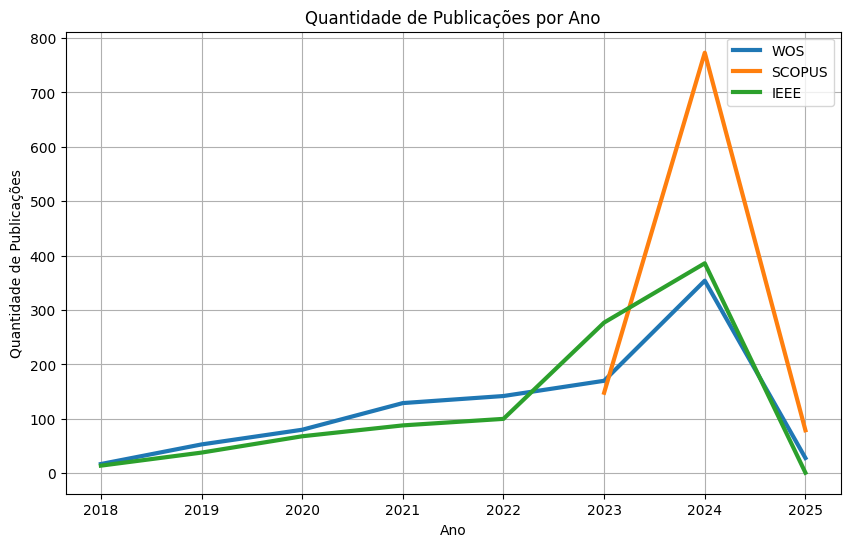
\includegraphics[width=10cm]{Comparativo_volume_de_publicações_impacto.png}
    {\\\footnotesize Fonte: Autoria Própria}
    \label{fig:2}
\end{figure}

%***** Subsecção da produtividade dos periódicos *****
\subsection{Análise da produtividade dos periódicos}

Com o objetivo de compreender melhor a origem das publicações e identificar os principais difusores de artigos sobre o tema, foi realizada a concatenação dos dados das três bases de dados. Em seguida, aplicou-se um agrupamento para analisar as fontes das publicações. Os resultados dessa análise estão representados no gráfico da Figura \ref{fig:3}.

\begin{figure}[H]
    \centering
    \caption{Análise quantitativa parcial de publicações por sua origem}
    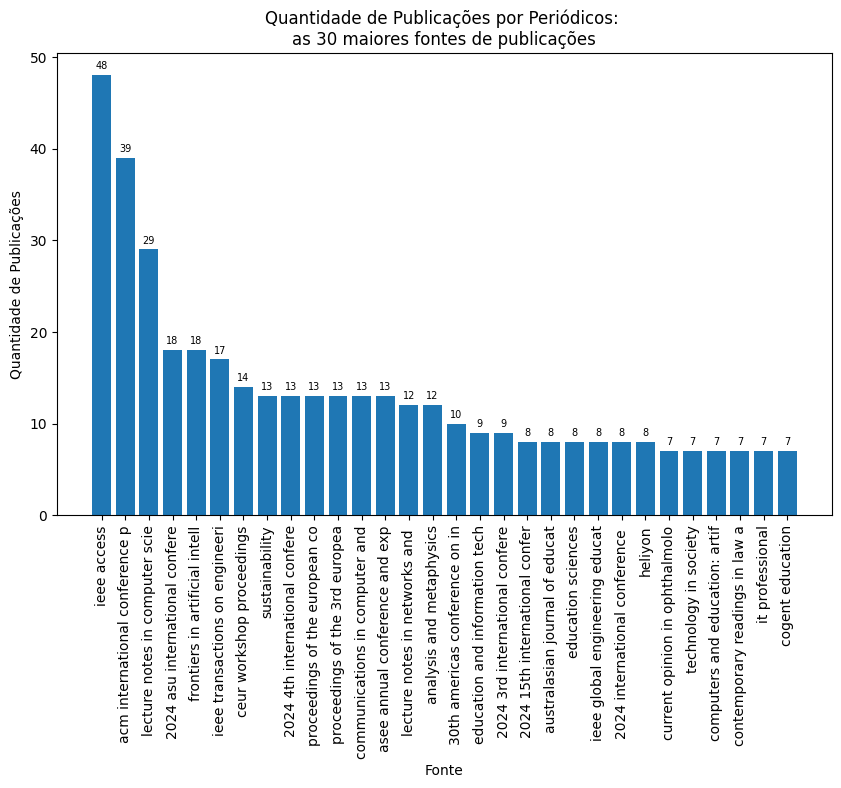
\includegraphics[width=10cm]{qtd_publicacoes_fonte.png}
    {\\\footnotesize Fonte: Autoria Própria}
    \label{fig:3}
\end{figure}

A análise da Figura \ref{fig:3} revela uma significativa dispersão das publicações entre diferentes periódicos. Embora os periódicos com maior índice de disseminação apresentem um número considerável de publicações, este é relativamente baixo quando comparado ao total de artigos relevantes publicados.

A tabela \ref{tab:resumo_qtd_publicacoes} apresenta a totalização dessas publicações, considerando a quantidade de periódicos associadas a cada total. Observa-se claramente que, à medida que o número de publicações por periódico diminui, aumenta o número de fontes que as publicam. Dessa forma, as fontes com menor número de publicações tornam-se menos relevantes no contexto do tema pesquisado \cite{lousada2012produccao}.

\begin{table}[H]
    \centering
    {\fontsize{6pt}{7pt}\selectfont
    \begin{tabular}{cccc}
        \hline
        Qtd. Publicações & Qtd. Fontes & Total Fontes & Total Publicações \\
        \hline
        \rowcolor{red!30} 48  & 1    & 1    & 48   \\
        \rowcolor{red!30} 39  & 1    & 2    & 87   \\
        \rowcolor{red!30} 29  & 1    & 3    & 116  \\
        \rowcolor{red!30} 18  & 2    & 5    & 152  \\
        \rowcolor{red!30} 17  & 1    & 6    & 169  \\
        \rowcolor{red!30} 14  & 1    & 7    & 183  \\
        \rowcolor{red!30} 13  & 6    & 13   & 261  \\
        \rowcolor{red!30} 12  & 2    & 15   & 285  \\
        \rowcolor{red!30} 10  & 1    & 16   & 295  \\
        \rowcolor{red!30} 9   & 2    & 18   & 313  \\
        \rowcolor{red!30} 8   & 6    & 24   & 361  \\
        \rowcolor{red!30} 7   & 9    & 33   & 424  \\
        \rowcolor{red!30} 6   & 12   & 45   & 496  \\
        \rowcolor{red!30} 5   & 12   & 57   & 556  \\
        \rowcolor{red!30} 4   & 27   & 84   & 664  \\
        \rowcolor{red!30} 3   & 81   & 165  & 907  \\
        2   & 252  & 417  & 1411 \\
        1   & 1427 & 1844 & 2838 \\
        \hline
        }
    \end{tabular}
    \caption{Tabela de publicações e periódicos com destaque para os periódicos relevantes.}
    \label{tab:resumo_qtd_publicacoes}
\end{table}

Na etapa seguinte, a análise de dispersão das publicações foi realizada com o objetivo de identificar os agrupamentos difusores, conforme previsto pela Lei de Bradford \cite{gracio2020analises} e \cite{lousada2012produccao}. Para isso, as fontes dos artigos foram organizadas em três grupos distintos, ordenados de acordo com a quantidade de publicações. A distribuição seguiu o critério de divisão do total de publicações em três partes iguais, resultando em um valor de referência de $2838/3 = 946$. Dessa forma, o núcleo de Bradford, que representa as fontes mais relevantes, corresponde ao conjunto de publicações até a linha destacada na Tabela \ref{tab:resumo_qtd_publicacoes}. Pode-se, então, afirmar que, para cada periódico pertencente à classe mais relevante, existem doze outros de menor relevância, evidenciando a concentração da produção científica em 165 periódicos de alto impacto.

Com base nas teorias dos núcleos difusores de Bradford, foi possível identificar um conjunto de periódicos de maior relevância, permitindo a redução da base original de 3.000 publicações para 891 artigos considerados pertinentes à análise.

%**** Subseção da produtividade dos autores ****
\subsection{Análise da produtividade dos autores}

Aplicando-se uma metodologia semelhante à descrita na subseção anterior, foi realizado o levantamento do volume de produção de cada autor em cada base de dados, conforme estabelecido na seção anterior. Os resultados parciais dessa análise são apresentados na Figura \ref{fig:4}.

\begin{figure}[H]
    \centering
    \caption{Totalização de publicações por autores}
    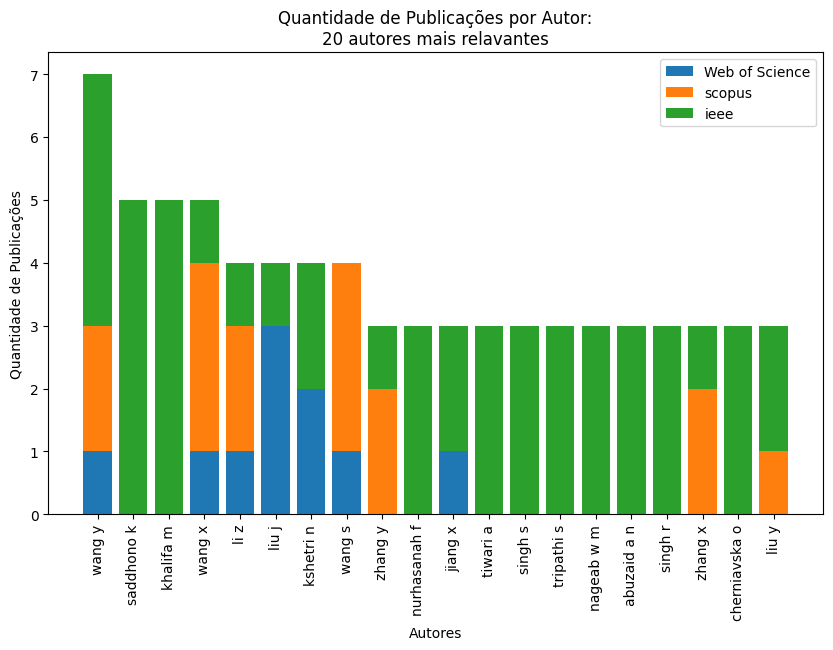
\includegraphics[width=10cm]{publicacoes_autores.png}
    \label{fig:4}
    {\\\footnotesize Fonte: Autoria Própria}
\end{figure}

O levantamento realizado identificou um total de 2.822 autores distribuídos em 891 artigos. De acordo com Lotka, conforme descrito por \textcite{melo2017bibliometria}, a produtividade científica tende a seguir um padrão no qual um pequeno grupo de autores é responsável pela maior parte das publicações, enquanto a maioria contribui com apenas um ou poucos artigos. Esse comportamento é evidenciado na Tabela \ref{tab:2}, onde 2.620 autores publicaram apenas um artigo, enquanto um único autor foi responsável por sete publicações, demonstrando a forte assimetria na distribuição da produção acadêmica sobre o tema.

\begin{table}[H]
    \centering
    \footnotesize
    \begin{tabular}{cccc}
        \hline
        Qtd. Publicações & Qtd. Autores & Total de Autores & Total de Participações em Publicações \\
        \hline
        \rowcolor{red!30} 7  & 1    & 1    & 7    \\
        \rowcolor{red!30} 5  & 3    & 4    & 22   \\
        \rowcolor{red!30} 4  & 4    & 8    & 38   \\
        \rowcolor{red!30} 3  & 18   & 26   & 92   \\
        \rowcolor{red!30} 2  & 176  & 202  & 444  \\
        1  & 2620 & 2822 & 3064  \\
        \hline
    \end{tabular}
    \caption{Distribuição das publicações por autor.}
    \label{tab:2}
\end{table}

A Tabela \ref{tab:2} mostra que, ao segmentar o grupo de autores com base no total de participações em publicações em três grupos de relevância ($3064/3\approx1021.33$), a última linha ultrapassava o limite de corte estabelecido. Tal corte auxiliou na redução ainda maior da base de dados de publicações, diminuindo o total para 257 artigos relevantes.

%***** Análise das palavras utilizadas *****
\subsection{Análise das palavras nos Títulos, Palavras-chaves e Resumos}

Com a redução das bases de dados, buscou-se identificar os principais temas discutidos nas publicações selecionadas. Para essa finalidade, foi realizada uma análise dos títulos, palavras-chave e resumos dos artigos. Em vez de aplicar diretamente a Lei de Zipf, conforme descrita por \textcite{guedes2005bibliometria}, optou-se por remover previamente os elementos estruturais da língua inglesa, como conjunções coordenativas e subordinativas, conjunções correlativas, artigos, preposições, pronomes, predeterminadores, verbos auxiliares, pronomes demonstrativos, advérbios e adjetivos possessivos. Esse procedimento garantiu a preservação apenas de estruturas linguísticas de maior carga semântica, incluindo substantivos, verbos principais, adjetivos descritivos, numerais e interjeições, facilitando a quantificação dos termos mais relevantes. Como resultado, foi possível inferir com maior precisão os tópicos predominantes abordados nos artigos analisados.

A Figura \ref{fig:5} apresenta a nuvem de palavras gerada a partir dos títulos, palavras-chave e resumos dos artigos selecionados. Nesse tipo de representação gráfica, os termos mais recorrentes são exibidos com maior destaque em relação aos demais. Para uma análise mais significativa, foram desconsideradas palavras intrinsecamente relacionadas ao escopo da pesquisa, como \textit{artificial, intelligence, AI, generative} e \textit{impact}, uma vez que derivam diretamente da seleção dos artigos. Observa-se, entretanto, a presença de termos associados a distintas áreas do conhecimento, tais como educação, tecnologia, marketing, mercado e literatura. Além disso, a identificação de substantivos menos frequentes, como desafios, ética, avaliação e potencial, sugere aspectos críticos e impactos relevantes dessa tecnologia em diferentes contextos.

\begin{figure}[H]
    \centering
    \caption{Totalização das palavras: Títulos, Palavras-Chave e Resumos}
    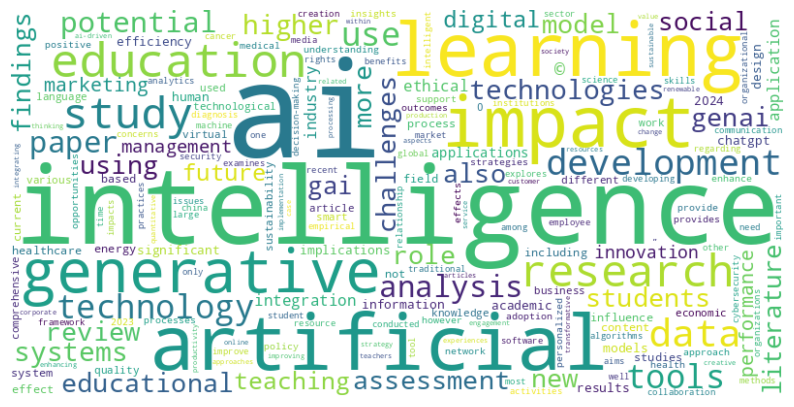
\includegraphics[width=11cm]{nuvem_palavras.png}
    \label{fig:5}
    {\\\footnotesize Fonte: Autoria Própria}
\end{figure}


%************************
% Considerações Finais **
%************************
\section{Considerações Finais}
\onehalfspacing
 O presente estudo realizou uma análise bibliométrica detalhada sobre as Inteligências Artificiais Generativas (IAGs), destacando os avanços científicos e os desafios enfrentados pela comunidade acadêmica. Por meio da aplicação de metodologias quantitativas, como as leis de Bradford, Lotka e Zipf, foi possível identificar padrões de disseminação do conhecimento, os principais periódicos e autores mais produtivos, além das áreas do conhecimento impactadas por essas tecnologias \cite{guedes2005bibliometria}. A pesquisa revelou um crescimento exponencial no volume de publicações sobre IAGs nos últimos anos, reforçando o interesse crescente nesse campo e a necessidade de uma organização criteriosa da produção científica.

 Os resultados indicam que, embora a distribuição da pesquisa sobre IAGs apresente padrões compatíveis com as Leis de Bradford e Lotka, a concentração de publicações nos principais periódicos e entre os autores mais produtivos ainda é relativamente baixa. Observa-se que a maior parte dos artigos está dispersa entre um grande número de periódicos e autores que publicaram apenas uma vez sobre o tema, sugerindo que os núcleos difusores e os pesquisadores mais influentes ainda estão em processo de formação. Essa característica pode ser explicada pela recente ascensão das IAGs, o que implica em um cenário acadêmico ainda fragmentado. No entanto, a análise dos dados sugere que essas concentrações estão começando a se consolidar, indicando uma possível estruturação futura da produção científica sobre o tema.

 A análise dos títulos, palavras-chave e resumos permitiu identificar os principais temas abordados nas publicações. Foram observadas fortes correlações entre IAGs e áreas como educação, tecnologia, marketing e mercado, além da recorrência de termos associados a desafios éticos e metodológicos, como avaliação, potencial e impacto. Essa análise semântica contribui para a identificação de tendências emergentes e lacunas na literatura, fornecendo um direcionamento para futuras investigações.
 
\printbibliography

\end{document}
